\documentclass{llncs}
\usepackage{graphicx}
\usepackage{placeins}
\usepackage{upgreek}
%
\begin{document}
\pagestyle{headings} 
\mainmatter
%
\title{Hybrid Approach Based on Combination of Backpropagation and Evolutionary Algorithms for Artificial Neural Networks Training by Using Mobile Devices in Distributed Computing Environment}
%
\author{Iliyan Zankinski, Maria Barova, Petar Tomov}
%
\authorrunning{Iliyan Zankinski} 
%
\tocauthor{Iliyan Zankinski, Maria Barova, Petar Tomov}
%
\institute{Institute of Information and Communication Technologies\\
Bulgarian Academy of Sciences\\
acad. G. Bonchev Str, Block 2, 1113 Sofia, Bulgaria\\
\email{iliyan@hsi.iccs.bas.bg}}
%
%Iliyan Zankinski iliyan@hsi.iccs.bas.bg
%Maria Barova m.barova@iit.bas.bg
%Petar Tomov p.tomov@iit.bas.bg 
%
\maketitle
%
\begin{abstract}
When Evolutionary Algorithms (EAs) are used for Artificial Neural Networks (ANNs) training, the most valuable advantage is the potential for this training to be done in parallel or even using distributed computing. With the capabilities of modern mobile devices, for example their use for distributed computations, they can be used much more extensively for scientific calculations. It is well known that distributed computing systems are limited by their communication bandwidth, because of network latency. In such environment some EAs are pretty suitable for distributed implementation. This is because of their high level of parallelism and relatively less intensive network communication needs. Subset of distributed computing is volunteer computing where users donate some of the computing power provided by devices under their control. This research proposes Android Live Wallpaper volunteer computing implementation of a system used for financial time series prediction. The forecasting module is organized as ANN, which is trained by hybrid combination of Backpropagation and EAs. 
\keywords{Artificial Neural Networks, Evolutionary Algorithms, Distributed Computing}
\end{abstract}
%
\section{Introduction}
%
ANNs are very common in the field of machine learning. In its nature ANN training is an optimization problem. When the searching space is too big EAs for global optimization as Genetic Algorithms (GAs) can be very suitable. In the last two decades there are alot of attempts to combine EAs based optimization with the ANNs training. This combination shows to be much more promising when it is implemented as distributed computing system [1,2,3]. With the rising popularity of the mobile devices a lot of new possibilities for distributed computing can be investigated. Successful desktop distributed computing projects [4,5] can be efficiently implemented on mobile devices. This idea can be applied on EA based ANN training into a mobile distributed computing environment [6]. In this paper genetic algorithm in combination with backpropagation artificial neural network training is described. The training is done on a mobile devices as active Android wallpaper application. In addition, the traditional ANN's sigmoid function is replaced by fading sinusoidal function. The successful application of this hybrid approach is documented by series of experiments.

This paper is organized as follows. Section 1 gives an overview of the problem  with a special emphasis on ANNs/GAs and their strengths/weaknesses when applied for the problem's solution. Section 2 introduces a distributed computing environment based on mobile devices. Experiments and results are presented in Section 3. The final Section 4 concludes and some further work suggestions are provided. 
%
\subsection{Financial Time Series Forecasting}
%
A time series is a collection of measurements made in a sequence through the time. There are many examples for time series like the sales of the specific stock in successive months, the average daily temperature at a particular location, the electricity consumption in a particular areal for successive seasons and many other. In the field of the finance, decision makers are in the position of taking very responsible steps during formation of investment strategy. To invest it means to take acceptable risk with expectation of certain amount of profit. The most important aspect of investment is the balance between risk taken and expected profit. On the currency market (FOREX) the main trading is done by exchanging currencies. Currency is the most volatile in price changing object of trading. During the process of trading on such market as FOREX decision makers needs to take three important decisions: 1. Price will go up or down; 2. What volume to buy or sell; 3. How long to keep the opened position. Even it sounds simple in fact it is very difficult to estimate price changing direction, because the huge amount of factors influence it. The order volume is directly related to amount of risk taken. High volume order can lead to high profit if price changing direction is well estimated, but it can lead to high loss in other case. How long to keep the opened position is related to make the profit even bigger or to make the loss as smaller as possible. Financial forecasting is most important for the traders on the currency market, because of the high price dynamics [2].
%
\subsection{Artificial Neural Networks}
%
Artificial Neural Network is a mathematical model inspired by research into the nature of the human brain. In common ANNs consists of five components: 

1. Network topology which is represented by a directed graph with arcs are referred as links.

2. A variable which represents the state of each node.

3. For each link a real value variable represents its weight.

4. A real value bias which is supplied to each node.

5. Node transfer function which determines the state of the node. The transfer function consists of an activation function (in most cases sigmoid or hyperbolic tangent). The activation function accepts sum of the inputs multiplied by the weights of the links between the node and the other nodes.

When the network is of a type feed-forward there is no recurrent links (graph without loops). The input nodes in such network does not have input arcs. In order the network to process information the input nodes should be supplied with values. After that the input information can be spread across the network. This action is known as feed-forward pass and it means that the other nodes are changing their state variable according to the propagation rules. The most used ANN topology is multilayer perceptron (MLP). In such network any path from an input node to an output node traverses the same number of arcs. A hidden layer in such ANN is a group of nodes which are not input, output and are on the same number of arcs distance from the input layer and the output layer. The network is fully connected if each node in particular layer is connected to each node in the previous layer. 

MLP has its popularity because of a few reasons. It was found that such networks generalize well in practical problems. When trained on a relatively sparse set of data points, they will often provide the right output for an input not presented in the training set. Secondly, gradient based training algorithms like backpropagation can be successfully applied in order to find a good set of weights in acceptable amount of time. The advantage of the backpropagation is calculation of the gradient of the error according to the weights for a given input by back propagating the error through the network. Of course there are some disadvantages in gradient based training algorithms. Gradient based training works well on simple training problems. When the problem complexity increases (most commonly because of the increased dimensionality and/or greater data complexity) the performance of the gradient based training falls off rapidly. 

The performance slow down seems come from the fact that complex spaces have nearly global optimum around the local optimum. Gradient search techniques tend to get trapped at local optimum. With a high enough gain (or momentum), backpropagation can escape these local optimum. However, it leaves them without knowing whether the next one it finds will be better or worse. When the nearly global optimum are well hidden among the local optimum, backpropagation can end up bouncing between local optimum without much overall improvement, thus making for very slow training. The second drawback of the gradient based training is the requirement the activation function differentiability. Backpropagation can not handle discontinuous  optimallty or discontinuous node activation functions.
%
\subsection{Genetic Algorithms}
%
Genetic Algorithms are meta heuristic for global optimization inspired from the ideas for the biological evolution. In common they have five components:

1. Approach for encoding the problem in the terms of chromosomes (population individuals).

2. An evaluation function which is used to determine survival capabilities of each chromosome.

3. A strategy for initial population initialization.

4. Set of operator applied over parent chromosomes in order reproduction to appear (in most cases – selection, crossover, mutation and/or domain specific genetic material recombination).

5. Set of parameters applied over the population and the operators.

\vspace{4 mm}

According these five common components GA operates in the following steps:

1. Initialization of the population (can be random or according some prior information).

2. Evaluation of each chromosome in the population. Relative ranking is the important result in this step.

3. Epochs of recombinations are executed until stopping criteria is met.

  \hspace{4 mm}3.1 Parents selection is generally stochastic but parent with better fitness value are preferred.
  
  \hspace{4 mm}3.2 Recombination operators are applied over the selected parents in order to produce children.
  
  \hspace{4 mm}3.3 Evaluation of the children is done in order to keep some of the in the population. In some cases full old population is replaced by the new generation, but in other cases only part of the new generation is kept. The elitism rule is applied when the best found individuals should survive until the end of the evolution.

If appropriate problem encoding and recombination operators are selected the algorithm is capable to produce better and better solutions, converging finally on results close to a global optimum. In more of the real practice problems (as the problem presented in this research) standard operators as crossover and mutation are sufficient. In such case GA can be used as black-box optimizer. It means that no specific knowledge of the problem domain is needed. As it is shown in this research by involving problem specific operators (crossover and mutation), the optimization efficiency can be improved. 

GA does not have a scaling problem as it is the case with ANN. Even more, GAs are very proper for parallel computing and even for distributed computing. It is like this because GA improves the current best candidate monotonically. It is done by keeping the best found candidates as part of the population while searching for better candidates continues. Also GAs are not threatened by trapping in a local optimum. The mutation and crossover operators can step from a valley across a hill to an even lower valley with no more difficulty than descending directly into a valley.
%
\section{Mobile Devices Distributed Computing}
%
%
\subsection{Neuron Activation Function proposal}
%
The most used activation functions in MLPs are the sigmoid function and the hyperbolic tangent function [7]. In this research sin function with exponent fading effect is proposed as neurons activation function (Fig. 1). Because of its fading effect neurons are more active in a specific input range. In the input is high positive or high negative the neuron stops acting as effect of over saturation.

Fading sine function is differentiable which is one of the common requirements in gradient based training of ANNs.
%
\begin{equation}
f(x) = \frac {\pi \sin(x)} { e^{ |x| }}
\end{equation}
%
\begin{figure}
	\centering
	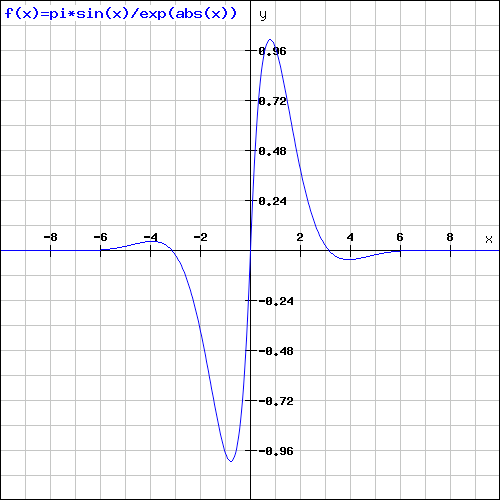
\includegraphics[width=7.88cm,height=7.88cm]{fig03.png}
	\caption{Proposed acrivation function.}
	\label{fig:Graph}
\end{figure}
\FloatBarrier
%
\begin{equation}
\frac{d}{dx}f(x) = \frac {\pi (|x|\cos x - x\sin x)} { |x| e^{ |x| } }
\end{equation}
%
\begin{equation}
\frac{d}{dx}f(x) = f(x + \pi) - f(x)
\frac{d}{dx}f(x) = f(x + \pi) + f(x)
\frac{d}{dx}f(x) = +\infty
\end{equation}
%
\begin{figure}
	\centering
	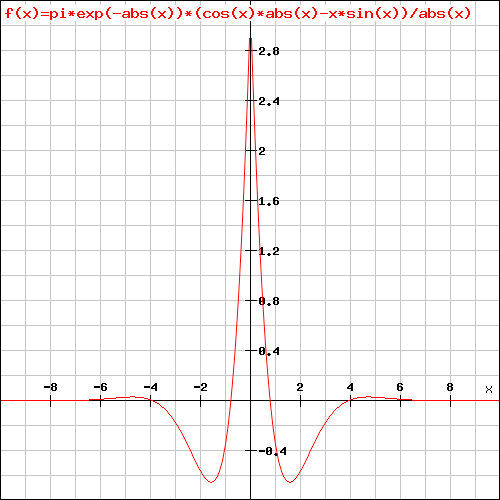
\includegraphics[width=7.88cm,height=7.88cm]{fig04.png}
	\caption{Proposed function derivative.}
	\label{fig:Graph}
\end{figure}
\FloatBarrier
%
\section{Experiments and Results}
%
%
\section{Conclusions}
%
Even that GA based ANN training is slower than back propagation when it is implemented as simultaneous computations in a distributed environment it can be efficient enough for practical use. Because modern mobile devices are used in 24/7 basis to use them as distributed computing network is very cost effective if the approach is based on donated computational power. As further development it will be interesting mobile devices distributed computing to be combined with supercomputers. The the central node it is possible to provide access of a super computer. Such hybrid infrastructure can provide interesting research and industrial challenges.
%
\section*{Acknowledgements}
%
This work was supported by private funding of Velbazhd Software LLC.
%
% ---- Bibliography ----
%
\begin{thebibliography}{}
%
\bibitem[1] {bal:zan:1}
Balabanov, T., Zankinski, I., Barova, M.:
Strategy for Individuals Distribution by Incident Nodes Participation in Star Topology of Distributed Evolutionary Algorithms.
Cybernetics and Information Technologies, Sofia, Bulgaria, vol. 16, no. 1, 80--88  (2016)
%
\bibitem[2] {bal:dob:1}
Balabanov, T., Zankinski, I., Dobrinkova, D.:
Time Series Prediction by Artificial Neural Networks and Differential Evolution in Distributed Environment.
International Conference on Large-Scale Scientific Computing, Sozopol, Bulgaria, Lecture Notes in Computer Science, vol. 7116, no. 1, 198--205  (2011)
%
\bibitem[3] {bal:1}
Balabanov, T.:
Heuristic Forecasting Approaches in Distributed Environment (in Bulgarian).
Proceedings of Anniversary Scientific Conference 40 Years Department of Industrial Automation, UCTM, Sofia, Bulgaria, 163--166 (2011)
%
\bibitem[4] {bal:2}
Balabanov, T.:
Distributed evolutional model for music composition by human-computer interaction.
Proceedings of International Scientific Conference UniTech15, University publishing house V. Aprilov, Gabrovo, Bulgaria, vol. 2, 389--392 (2015)
%
\bibitem[5] {bal:3}
Balabanov, T.:
Avoiding Local Optimums in Distributed Population based Heuristic Algorithms (in Bulgarian).
Proceedings of XXIII International Symposium Management of energy, industrial and environmental systems, John Atanasoff Union of Automation and Informatics, Sofia, Bulgaria, 83--86 (2015)
%
\bibitem[6] {bal:zan:2}
Balabanov, T., Zankinski, I., Barova, M.:
VitoshaTrade Distributed Computing Android Wallpaper.
https://github.com/TodorBalabanov/VitDisComp Sofia, Bulgaria  (2017)
%
\bibitem[7] {kar:veh:1}
Karlik, B, Vehbi, A.:
Performance Analysis of Various Activation Functions in Generalized MLP Architectures of Neural Networks.
International Journal of Artificial Intelligence And Expert Systems (IJAE), vol. 1, no 4, 111--122 (2011) 
%
\end{thebibliography}
\end{document}
